% Universidade Aberta
% Template TeX para relatório de trabalhos
% 2024
%
%
% Dados para a capa
\newcommand{\Titulo}{Tarefa 4.2}
\newcommand{\Ano}{2024}
\newcommand{\Autor}{Hugo Gonçalves}
%
%
\documentclass[12pt,a4paper,final]{article}
\usepackage{csquotes}
\usepackage[portuguese]{babel}
\usepackage{polyglossia}
\setdefaultlanguage{portuguese}
\usepackage{graphicx}
\graphicspath{ {./images/} }
\usepackage[a4paper,top=3cm,bottom=3cm,left=3.5cm,right=2cm]{geometry}
\usepackage{booktabs}
\usepackage{newtxtext}
\usepackage{newtxmath}
\usepackage[pdfauthor=\Autor,
    pdftitle=\Titulo,
    colorlinks=true,
    linkcolor=black,
    citecolor=black,
    bookmarksopen=true,
    breaklinks=true]{hyperref}
\hypersetup{colorlinks, citecolor=black, urlcolor=black}
\usepackage{bookmark}
\usepackage{float}
\renewcommand{\baselinestretch}{1.5}
\begin{document}
    \title{\Titulo}
    \author{\Autor}
    \date{\Ano}
    \pagenumbering{gobble}
    \begin{titlepage}
        \begin{center}
            \vspace*{4cm}

            \textbf{\large UNIVERSIDADE ABERTA}

            \textbf{\large UNIVERSIDADE DE TRÁS-OS-MONTES E ALTO DOURO}

            \vspace{1cm}

            \begin{minipage}{0.4\textwidth}
                \centering
                
\includegraphics[width=0.8\textwidth]{uab}
            \end{minipage}
            \begin{minipage}{0.4\textwidth}
                \centering
                
\includegraphics[width=0.8\textwidth]{utad}
            \end{minipage}

            \vspace{1.5cm}

            \textbf{\large \Titulo}

            \vspace{1.5cm}

            \textbf{\large \Autor}

            \vspace{2cm}

            \textbf{\large Mestrado em Engenharia Informática e Tecnologia Web}
            \vfill
            \textbf{\Ano}
        \end{center}
    \end{titlepage}
    \renewcommand{\contentsname}{Índice}
    \cleardoublepage
    \pagenumbering{roman}
    \tableofcontents
    \newpage
    \listoffigures
    \newpage
    \cleardoublepage
    \pagenumbering{arabic}


    \section{Introdução}\label{sec:introducao}
    Anteriormente, na Tarefa 3.2, o \textit{frontend} tinha sido evoluído para conter as entidades Patrocinador e Especialista.
    No decorrer dessa tarefa, o \textit{backend} foi atualizado, utilizando \textit{flags} para indicar se um dado utilizador era um patrocinador ou especialista.
    Assim, no decorrer da presente atividade, reverteram-se estas alterações no \textit{backend} e foram criados dois modelos específicos bem como todas as rotas necessárias.
    Além da adição das entidades referidas, foi também adicionado o \textit{Swagger UI}.


    \section{Rotas}\label{sec:patrocinador}
    Para ambas as entidades, foram adicionadas as rotas base CRUD.
    As novas entidades foram consideradas, também, utilizadores, pelo que podem ser utilizadas para aceder à plataforma.

    \subsection{Patrocinador}\label{subsec:patrocinador}
    \begin{figure}[H]
        \centering
        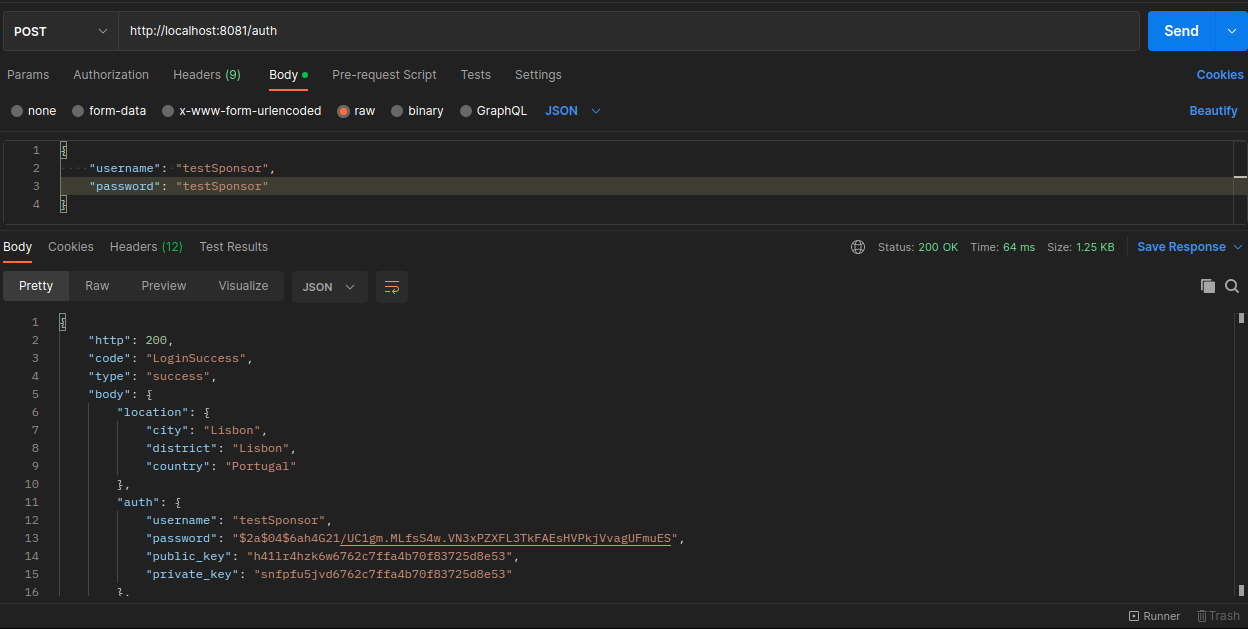
\includegraphics[width=0.9\textwidth]{login_sponsor}
        \caption{Patrocinador - Acesso}
        \label{fig:login_sponsor}
    \end{figure}

    \begin{figure}[H]
        \centering
        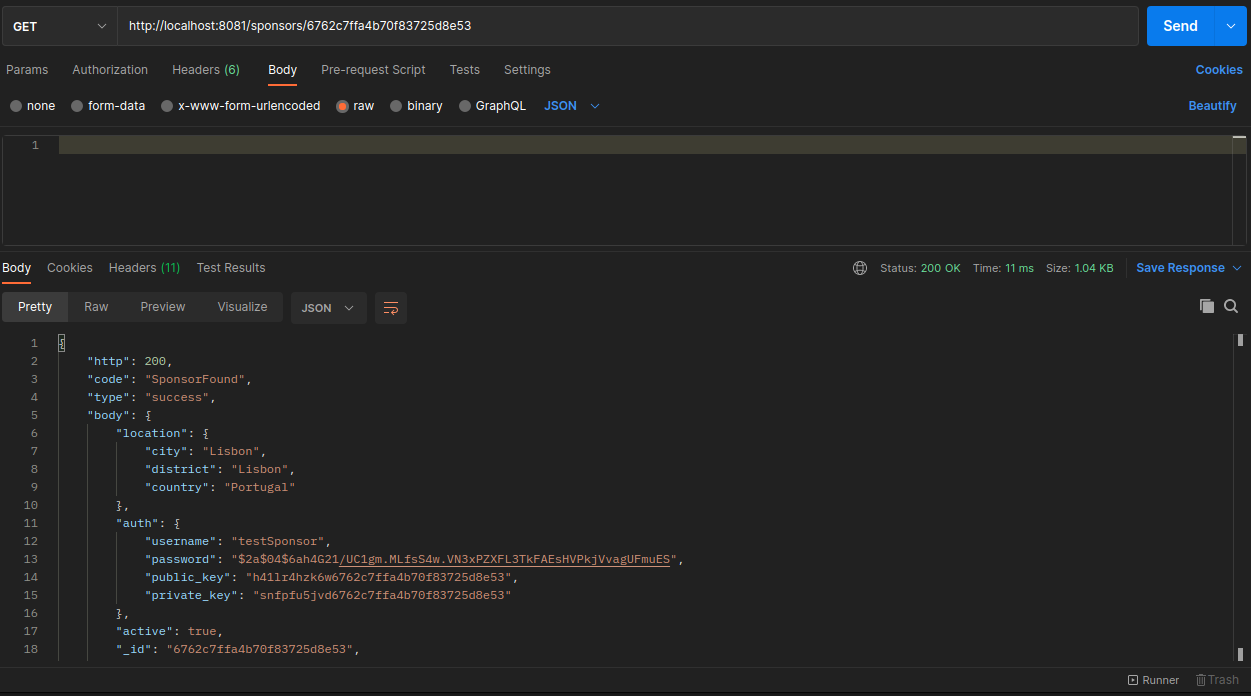
\includegraphics[width=0.9\textwidth]{get_sponsor}
        \caption{Patrocinador - Leitura}
        \label{fig:get_sponsor}
    \end{figure}

    \begin{figure}[H]
        \centering
        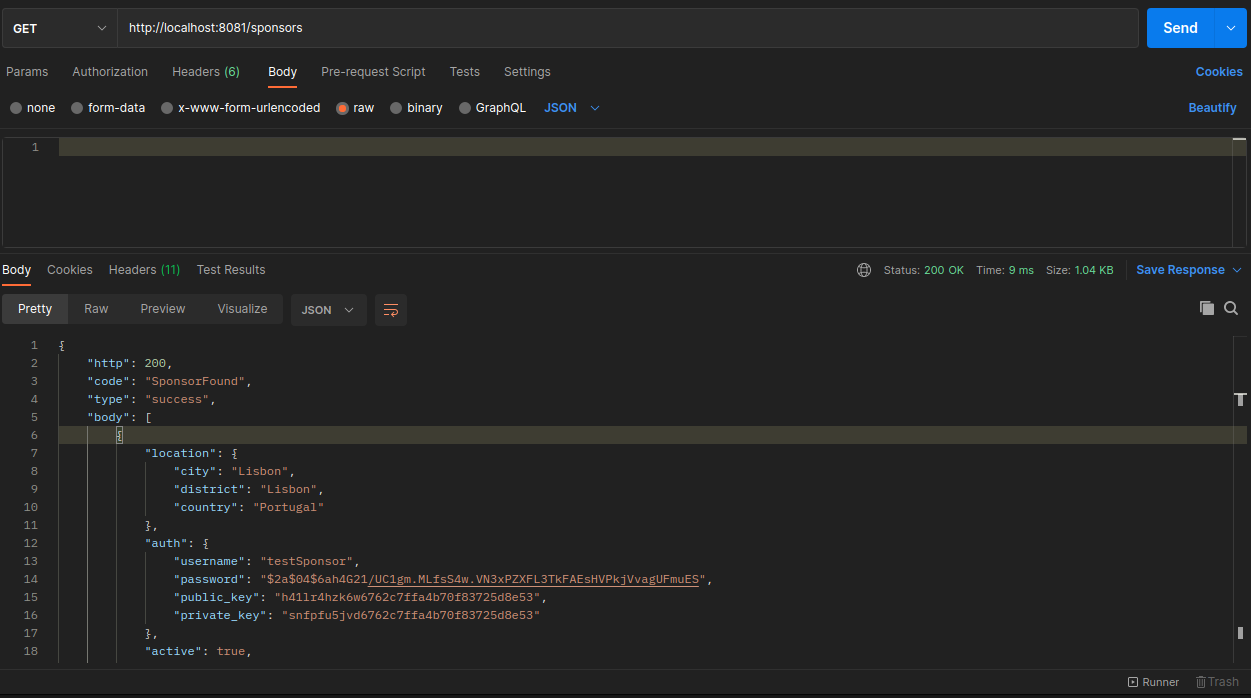
\includegraphics[width=0.9\textwidth]{get_sponsors}
        \caption{Patrocinadores - Leitura}
        \label{fig:get_sponsors}
    \end{figure}

    \begin{figure}[H]
        \centering
        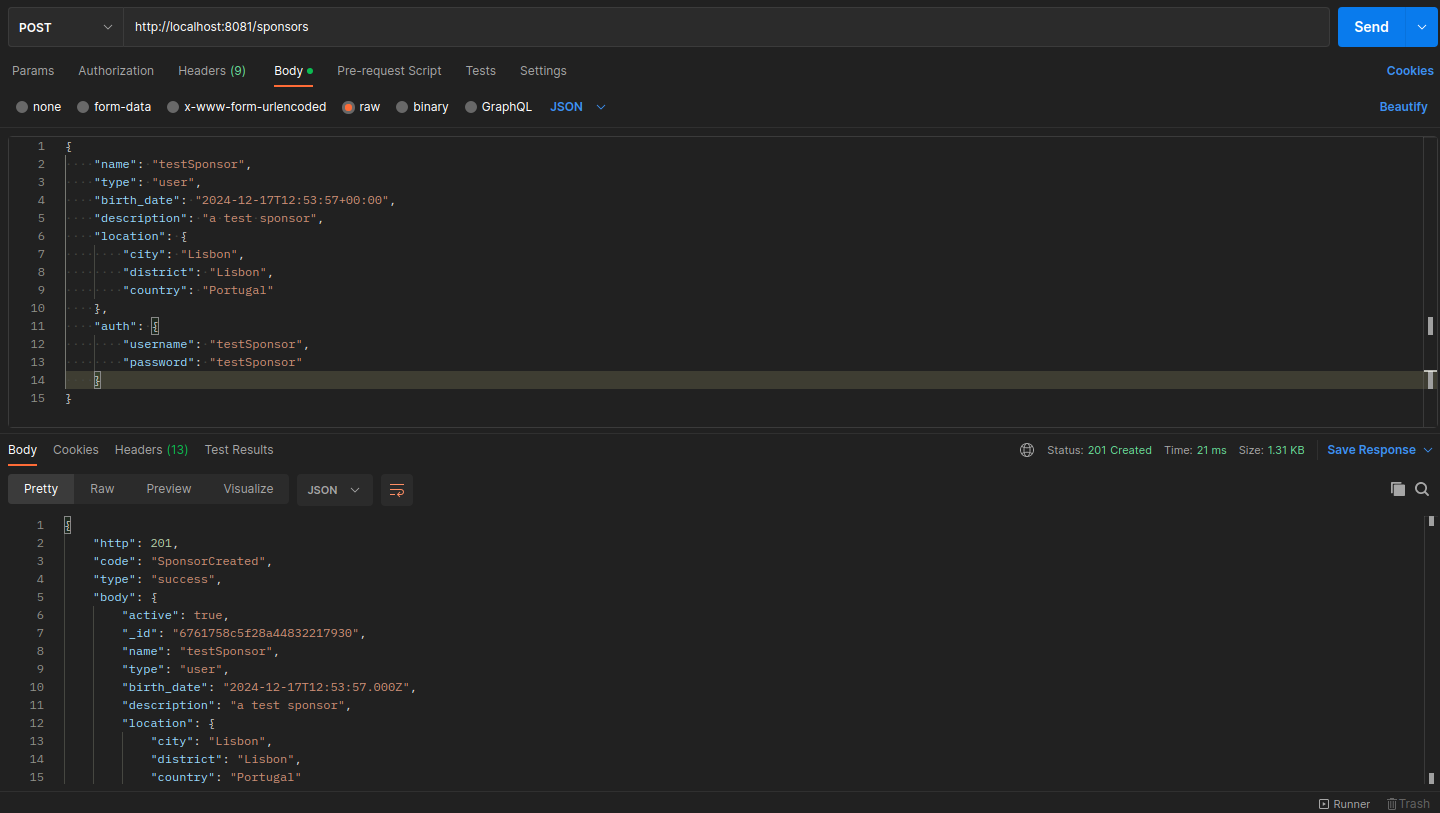
\includegraphics[width=0.9\textwidth]{cr_sponsor}
        \caption{Patrocinador - Criação}
        \label{fig:cr_sponsor}
    \end{figure}

    \begin{figure}[H]
        \centering
        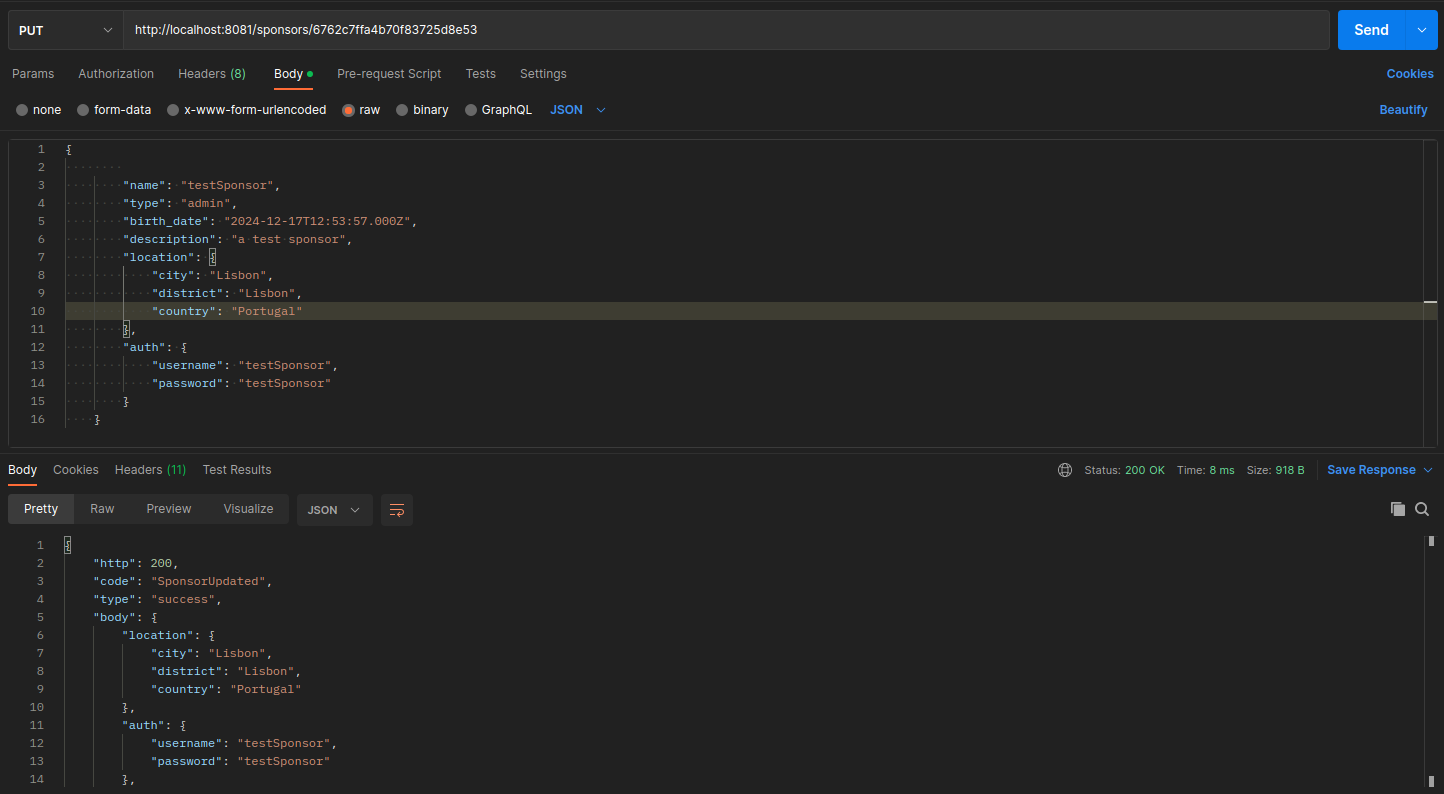
\includegraphics[width=0.9\textwidth]{update_sponsor}
        \caption{Patrocinador - Atualização}
        \label{fig:update_sponsor}
    \end{figure}

    \begin{figure}[H]
        \centering
        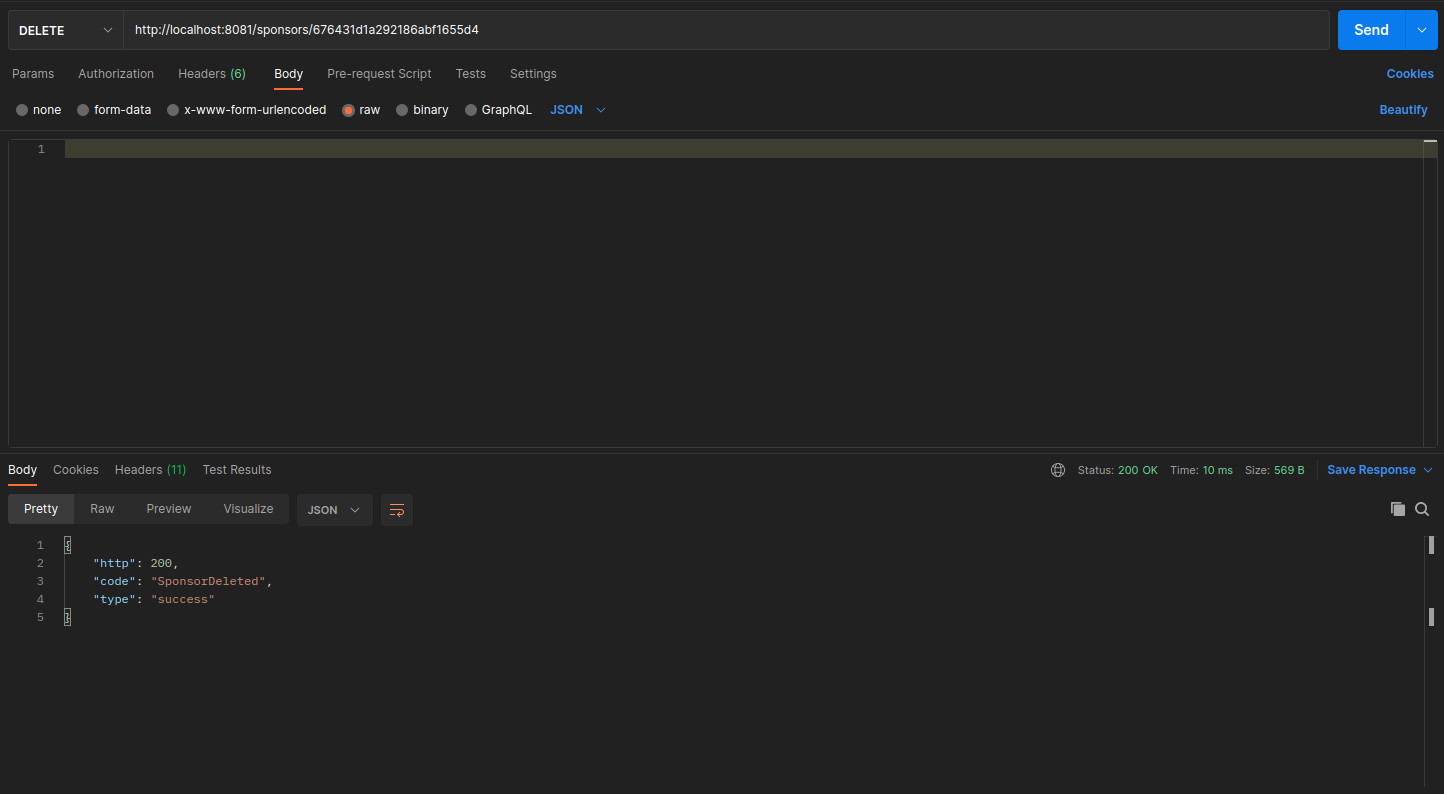
\includegraphics[width=0.9\textwidth]{del_sponsor}
        \caption{Patrocinador - Remoção}
        \label{fig:del_sponsor}
    \end{figure}

    \subsection{Especialista}\label{subsec:especialista}
    \begin{figure}[H]
        \centering
        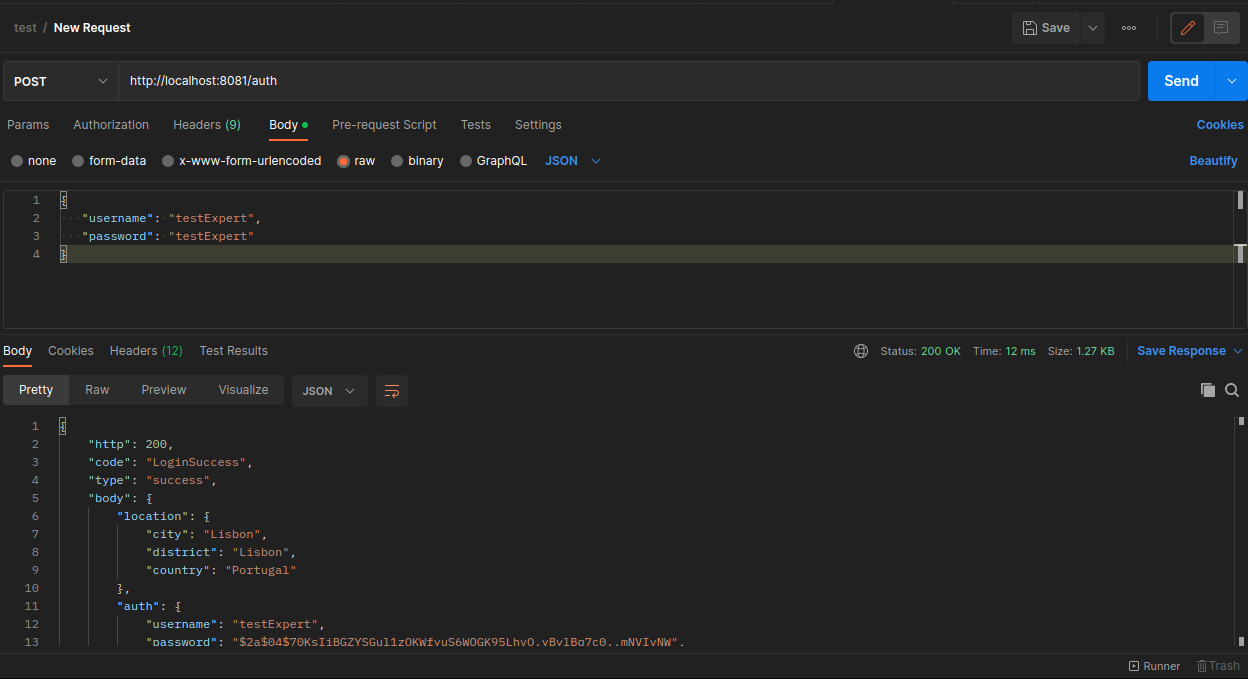
\includegraphics[width=0.9\textwidth]{login_expert}
        \caption{Especialista - Acesso}
        \label{fig:login_expert}
    \end{figure}

    \begin{figure}[H]
        \centering
        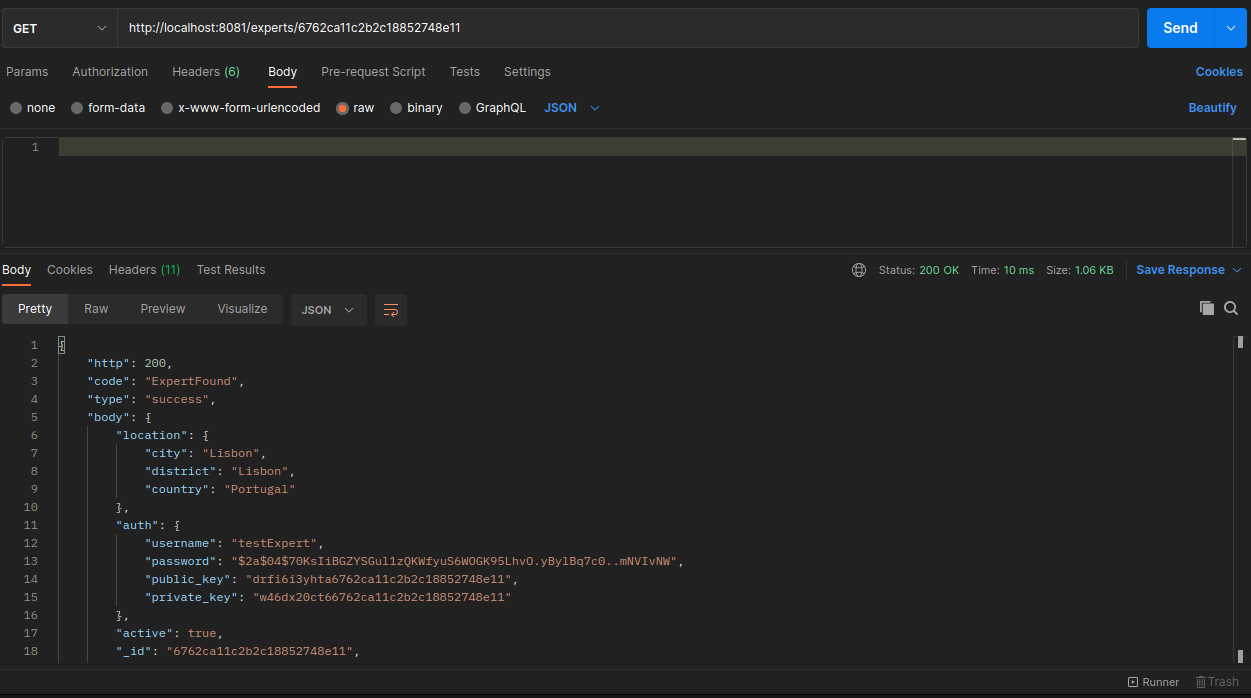
\includegraphics[width=0.9\textwidth]{get_expert}
        \caption{Especialista - Leitura}
        \label{fig:get_expert}
    \end{figure}

    \begin{figure}[H]
        \centering
        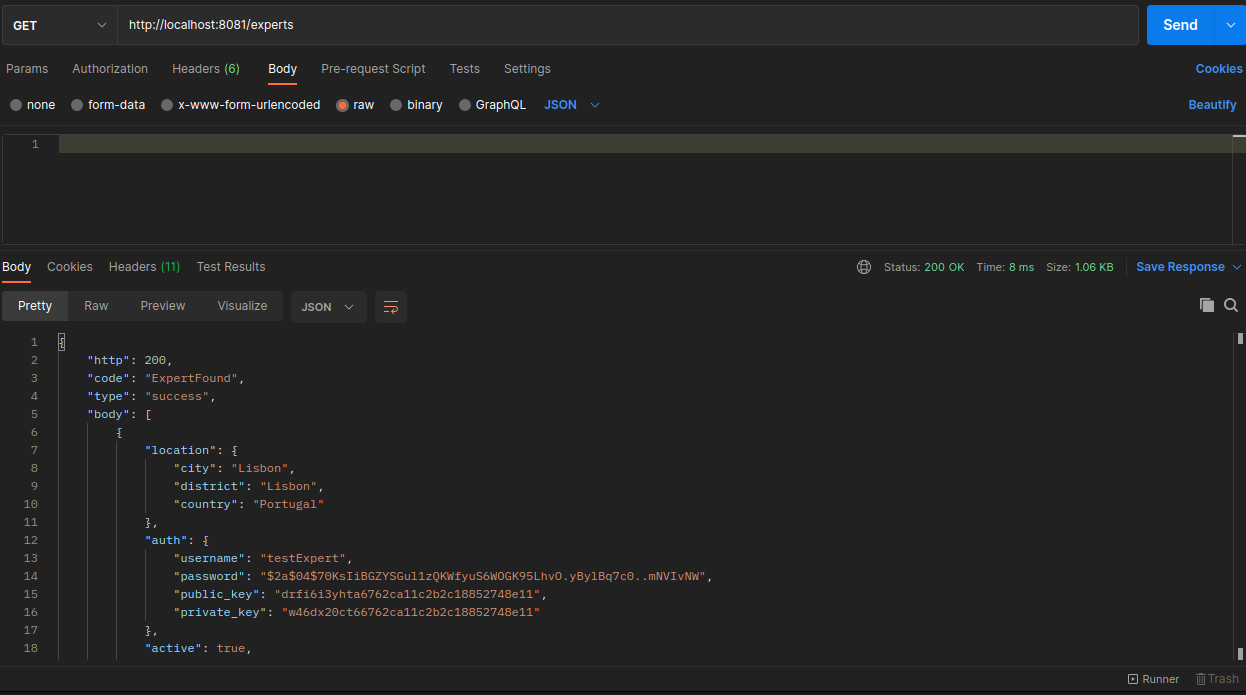
\includegraphics[width=0.9\textwidth]{get_experts}
        \caption{Especialistas - Leitura}
        \label{fig:get_experts}
    \end{figure}

    \begin{figure}[H]
        \centering
        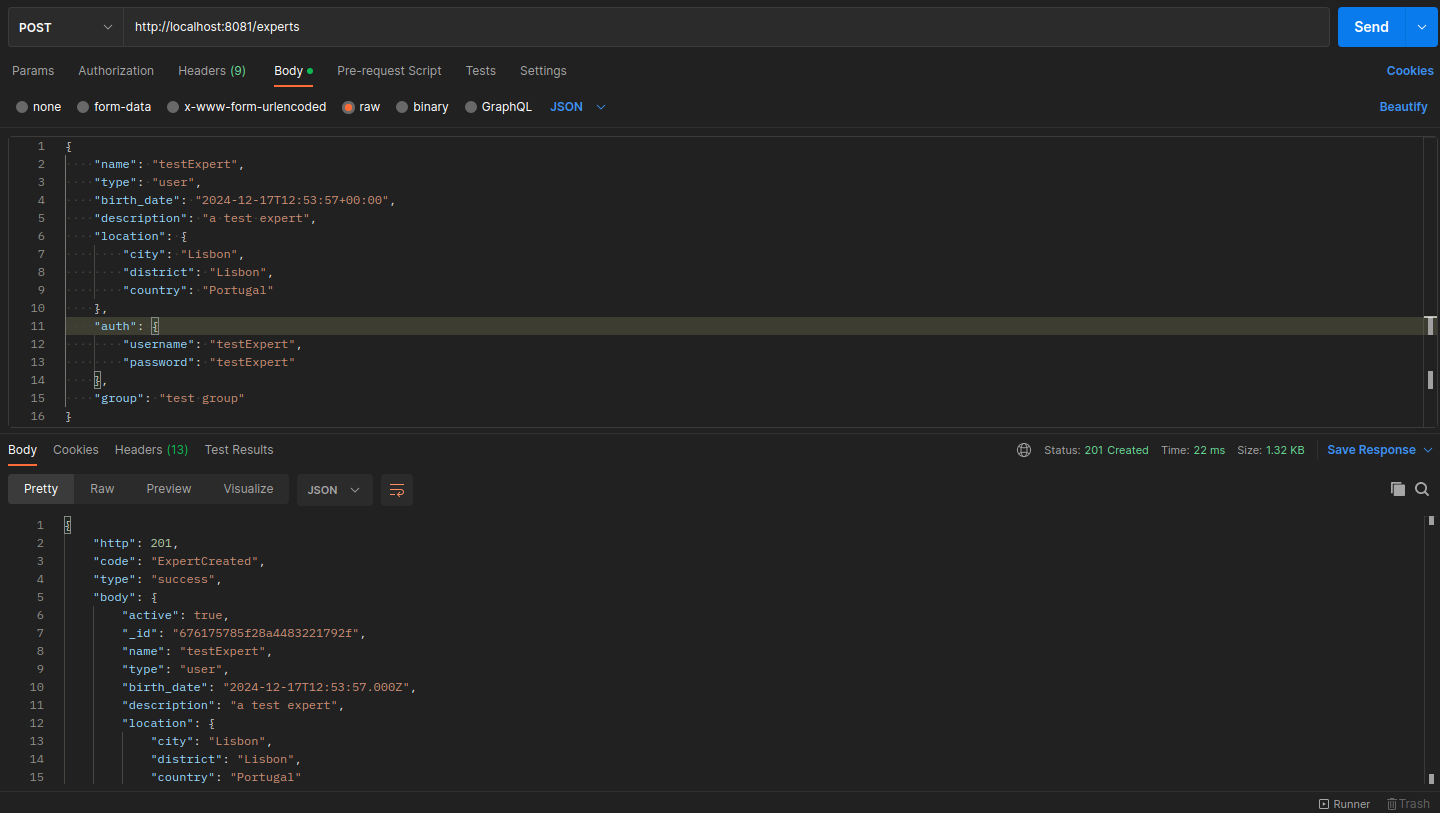
\includegraphics[width=0.9\textwidth]{cr_expert}
        \caption{Especialista - Criação}
        \label{fig:cr_expert}
    \end{figure}

    \begin{figure}[H]
        \centering
        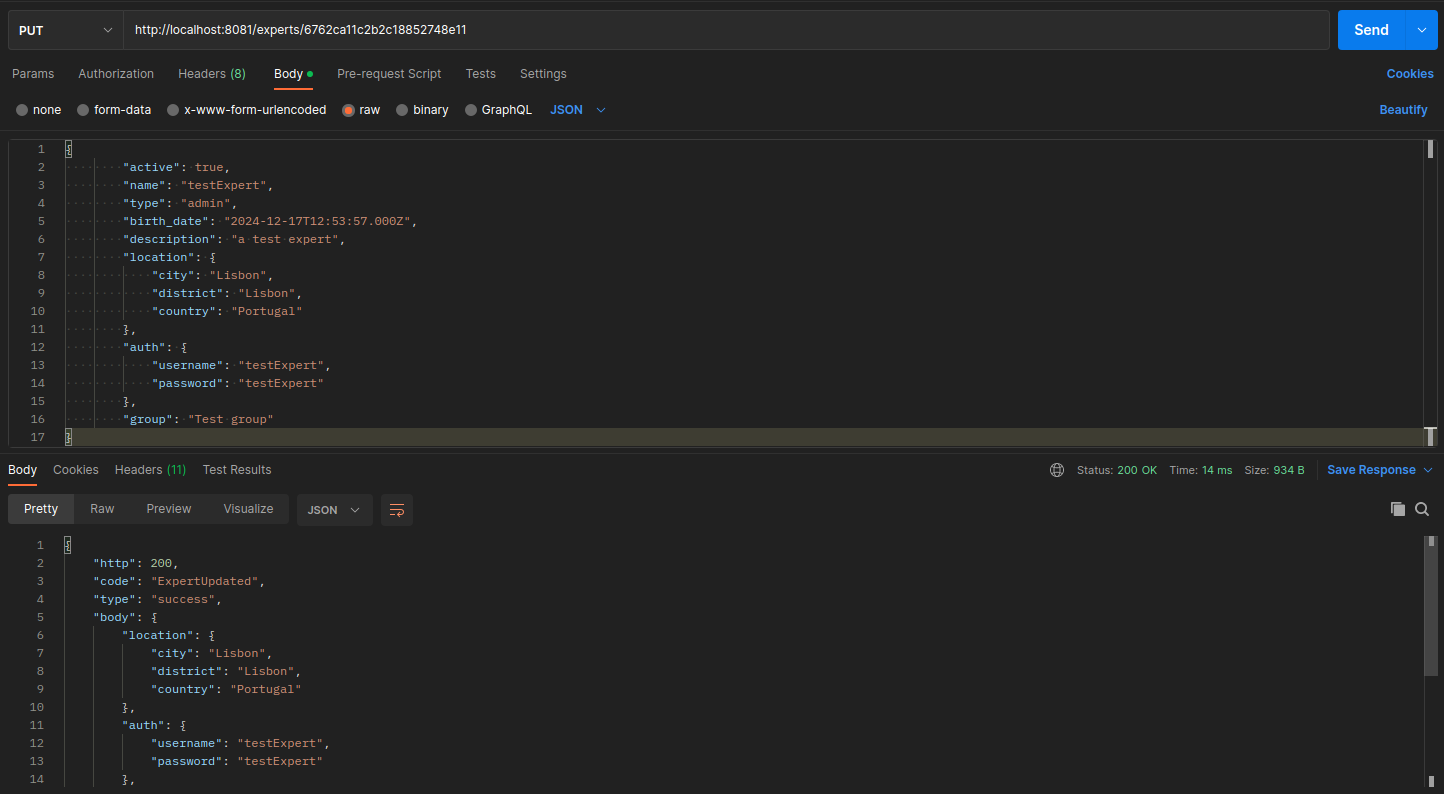
\includegraphics[width=0.9\textwidth]{update_expert}
        \caption{Especialista - Atualização}
        \label{fig:update_expert}
    \end{figure}

    \begin{figure}[H]
        \centering
        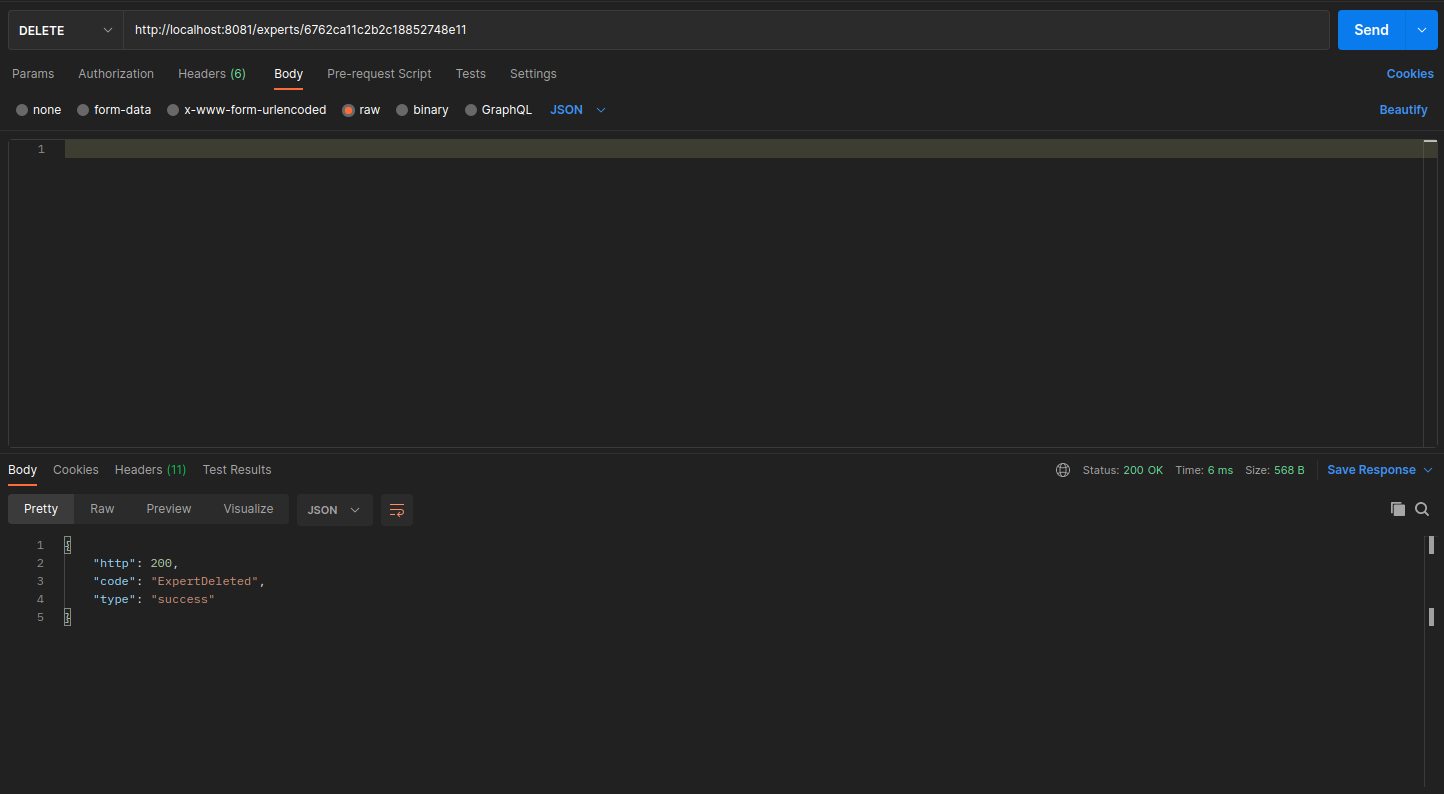
\includegraphics[width=0.9\textwidth]{del_expert}
        \caption{Especialista - Remoção}
        \label{fig:del_expert}
    \end{figure}

    \newpage
    \appendix
    \section*{Anexo A}
    O repositório onde se poderá acompanhar esta atividade está disponível neste \underline{\href{https://github.com/2100562/MiniProj3}{link}}.

    \newpage
    \section*{Anexo B}
    O \textit{Swagger UI} poderá ser acedido em <proto>://<hostname>:<port>/api-docs.
\end{document}
